\section{شرح پروژه}

\subsection{تغییرات نسبت به پروپوزال اولیه}

\section{طراحی و پیاده سازی}
در این پروژه ما با استفاده از 
\href{https://labcenter.s3.amazonaws.com/downloads/iotHelp.pdf}{iot-builder}
یک 
\subsection{شماتیک مدار}
شماتیک مدار را در شکل زیر مشاهده می‌کنید. در این مدار یک برد 
\lr{Arduino Yun}
که برای کاربرد‌های 
\lr{iot}
مناسب است و سه سنسور
\lr{LM35DZ}
تعبیه شده است که سنسور‌های دما هستند اما ما از آن‌ها به عنوان سنسور تشخیص گاز استفاده می‌کنیم. در پروپوزال ما سنسور‌های واقعی اندازه‌گیری گاز 
\lr{MQ-7}
و 
\lr{MQ-2}
و
\lr{MQ-135}
را استفاده کرده بودیم اما چون این سنسور‌ها در 
\lr{Proteus}
نبودند ما از سنسور‌های جایگزین اندازه‌گیری دما استفاده کردیم.
\begin{figure}[h!]
	\centering		
	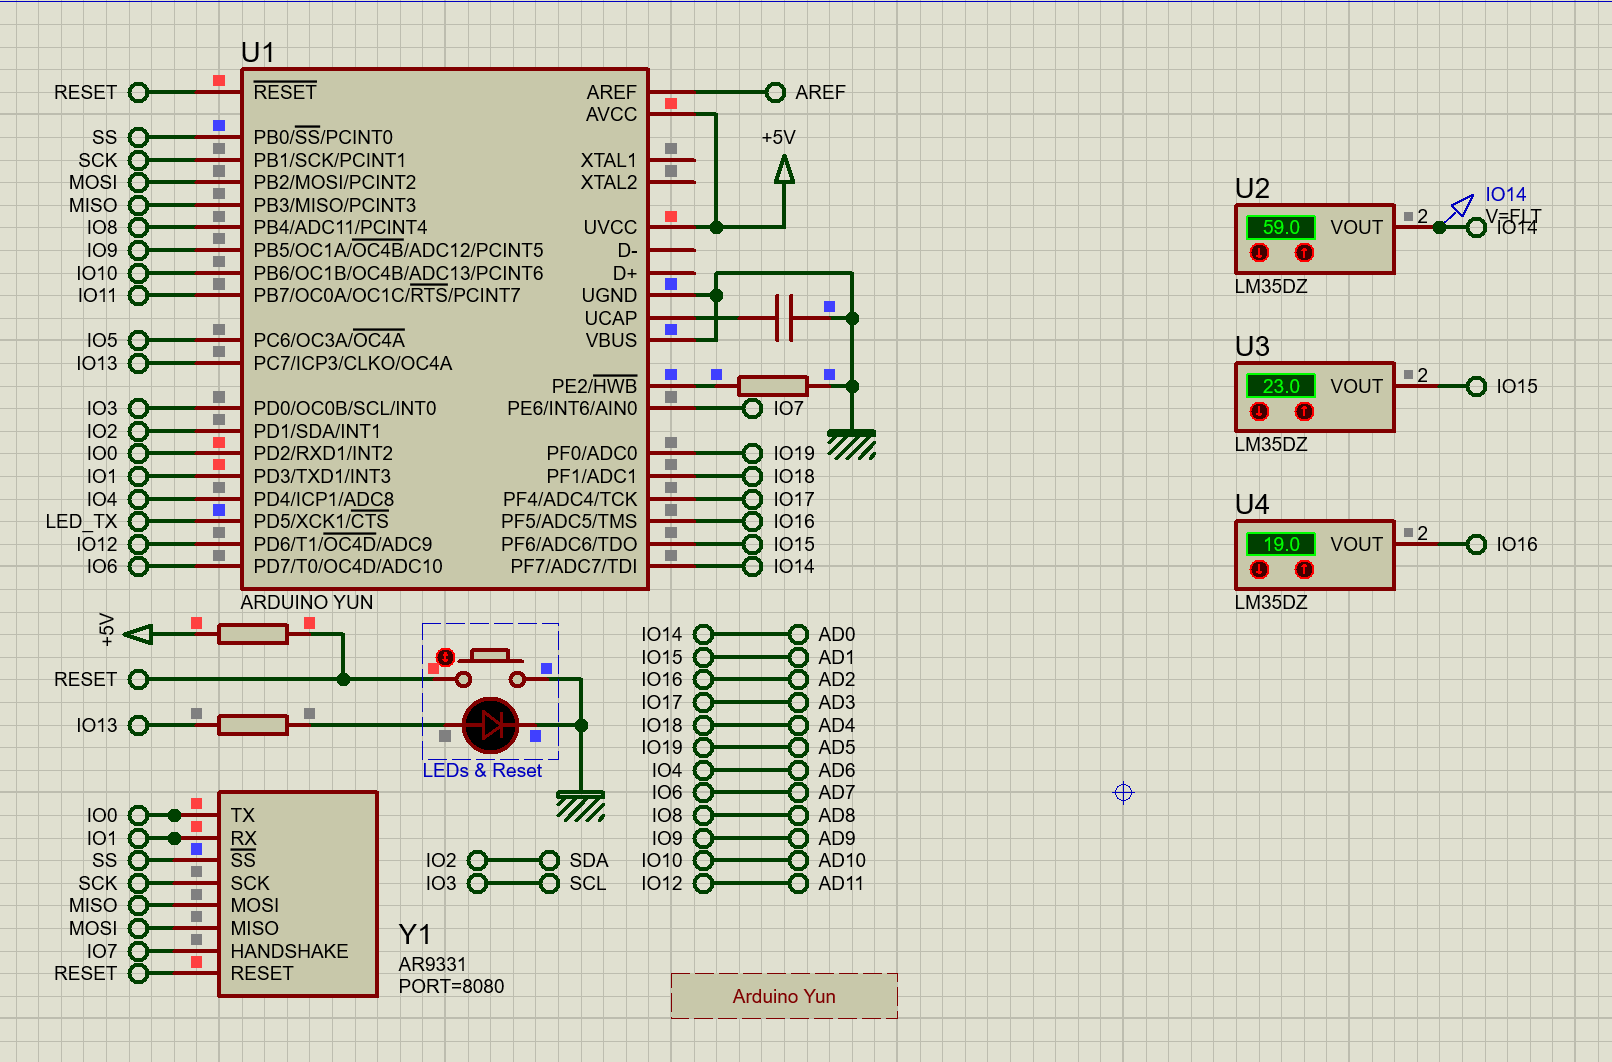
\includegraphics[width=\linewidth]{figs/circuit.png}
	\caption{شماتیک مدار}
\end{figure}

\subsection{اپلیکیشن گوشی}
برای طراحی اپلیکیشن گوشی ما از قابلیت‌های 
\lr{Visual Designer}
استفاده کردیم و کنترلر‌های 
\lr{iot}
زیر را 
\subsection{}


\section{ابزار‌های استفاده شده}


\section{سیمولیشن و نتایج}


